\newcommand{\figuraTemperaturaSolar}{%
\begin{figure}[H]
    \centering
    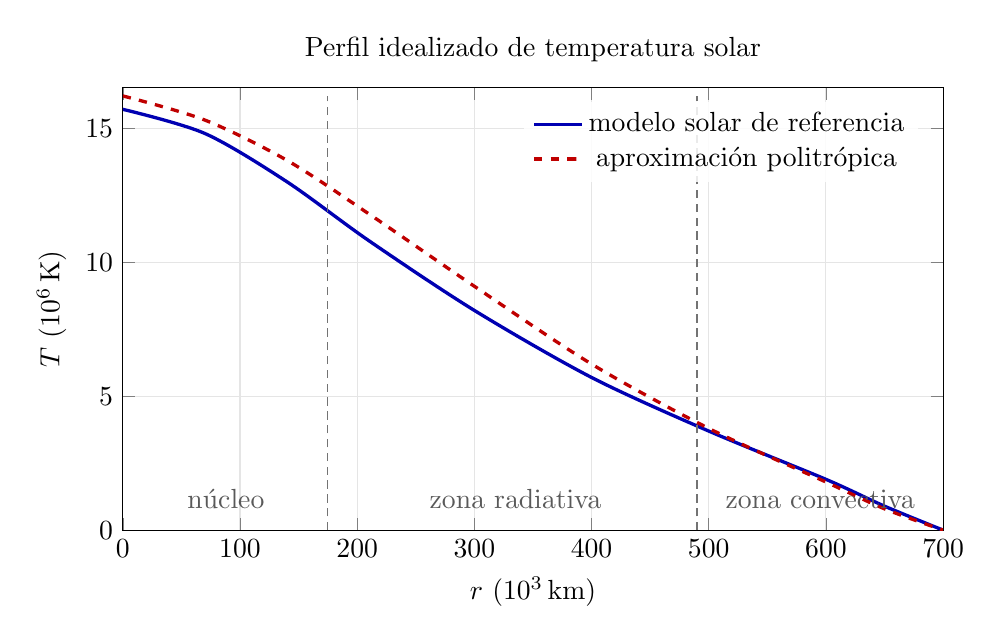
\begin{tikzpicture}
        \begin{axis}[
            width=12cm,
            height=7.2cm,
            xmin=0,xmax=700,
            ymin=0,ymax=16.5,
            xlabel={$r$ ($10^3\,\mathrm{km}$)},
            ylabel={$T$ ($10^6\,\mathrm{K}$)},
            title={Perfil idealizado de temperatura solar},
            grid=major,
            grid style={gray!20},
            legend style={at={(0.97,0.97)},anchor=north east,
                          draw=none,fill=white,fill opacity=0.85,
                          text opacity=1}]

            \addplot[very thick,blue!70!black,smooth]
                coordinates {
                    (0,15.7) (70,14.8) (140,13.0) (210,10.8)
                    (300,8.2) (400,5.7) (500,3.7) (600,1.9)
                    (650,0.9) (700,0.006)
                };
            \addlegendentry{modelo solar de referencia}

            \addplot[very thick,red!75!black,dashed,smooth]
                coordinates {
                    (0,16.2) (70,15.3) (140,13.8) (210,11.8)
                    (300,9.1) (400,6.2) (500,3.8) (600,1.8)
                    (650,0.8) (700,0.006)
                };
            \addlegendentry{aproximación politrópica}

            \draw[densely dashed,black!55]
                (axis cs:175,0)--(axis cs:175,16.2);
            \draw[densely dashed,black!55]
                (axis cs:490,0)--(axis cs:490,16.2);

            \node[anchor=south,text=black!65]
                at (axis cs:88,0.45) {núcleo};
            \node[anchor=south,text=black!65]
                at (axis cs:335,0.45) {zona radiativa};
            \node[anchor=south,text=black!65]
                at (axis cs:595,0.45) {zona convectiva};
        \end{axis}
    \end{tikzpicture}
    \caption{Comparación esquemática entre un perfil solar de referencia y
    una aproximación politrópica. El acuerdo mejora en la envolvente
    convectiva, donde el transporte es aproximadamente adiabático.}
    \label{fig:temperatura-solar}
\end{figure}%
}